% Template for Cogsci submission with R Markdown

% Stuff changed from original Markdown PLOS Template
\documentclass[10pt, letterpaper]{article}

\usepackage{cogsci}
\usepackage{pslatex}
\usepackage{float}
\usepackage{caption}

% amsmath package, useful for mathematical formulas
\usepackage{amsmath}

% amssymb package, useful for mathematical symbols
\usepackage{amssymb}

% hyperref package, useful for hyperlinks
\usepackage{hyperref}

% graphicx package, useful for including eps and pdf graphics
% include graphics with the command \includegraphics
\usepackage{graphicx}

% Sweave(-like)
\usepackage{fancyvrb}
\DefineVerbatimEnvironment{Sinput}{Verbatim}{fontshape=sl}
\DefineVerbatimEnvironment{Soutput}{Verbatim}{}
\DefineVerbatimEnvironment{Scode}{Verbatim}{fontshape=sl}
\newenvironment{Schunk}{}{}
\DefineVerbatimEnvironment{Code}{Verbatim}{}
\DefineVerbatimEnvironment{CodeInput}{Verbatim}{fontshape=sl}
\DefineVerbatimEnvironment{CodeOutput}{Verbatim}{}
\newenvironment{CodeChunk}{}{}

% cite package, to clean up citations in the main text. Do not remove.
\usepackage{apacite}

% KM added 1/4/18 to allow control of blind submission


\usepackage{color}

% Use doublespacing - comment out for single spacing
%\usepackage{setspace}
%\doublespacing


% % Text layout
% \topmargin 0.0cm
% \oddsidemargin 0.5cm
% \evensidemargin 0.5cm
% \textwidth 16cm
% \textheight 21cm

\title{Caregiver reconstruction of children's errors: the preservation of
complexity in language (improve title)}


\author{Madeline Meyers \and Daniel Yurovsky \\
        \texttt{\{mcmeyers, yurovsky\}@uchicago.edu} \\
       Department of Psychology \\ University of Chicago}

\begin{document}

\maketitle

\begin{abstract}
Why do languages change? One possibility is they evolve due to two
competing pressures: one, for the language to be easily transmitted to
new generations---and hence simple---and another, for the language to be
a useful, descriptive form of communication---and hence more complex.
However, few studies have explored these pressures in the most frequent
language learners: children. Conventional iterated learning studies
focus on the transmission of a novel language from one adult to the
next. However, this ignores one of the important features of language
learning, namely, receiving feedback. In this study, 120 adults on
Mechanical Turk participated in a conventional iterated learning task.
Their results were replicated with a larger sample of 480 adults.
Participant's performances indicate that complexity decreases in the
language over generations of transmission. 960 adults participated in a
third experiment, where half of the participants represented parent or
caregivers, who added a process of editing into generational
transmission (this all needs to be re-written and re-worded). Results
show that adding this error-correcting participant allows a greater
level of complexity to be retained in the language compared with having
a sole language learner/transmitter.

\textbf{Keywords:}
communication; language acquisition; language evolution; iterated
learning
\end{abstract}

\section{Introduction}\label{introduction}

How do you ask a group of people where they are going in Spanish? In
Spain, the answer depends on the group: you might ask ``Donde van
ustedes?'' of a group of work colleagues, but to address your friends,
you use the informal ``Donde váis vosotros?'' instead. In Mexican
Spanish, this distinction has disappeared, and the ``ustedes'' form is
used exclusively. Why did Spanish change in this way, simplifying and
shedding the formal second person plural? Why do languages change at
all? One working theory is that languages evolve to adapt to two dynamic
competing pressures: one, to be easily transmitted and learned (and
hence simple), and another, to be a descriptive and effective system for
communication (and hence complex) (Lupyan \& Dale, 2010).

When children are learning language, they often make simplification
errors (Bowerman, 1982). If a child is asking for some milk, they may
ask for a ``baba'' (bottle). Thus, the child has coined a new word,
which her parents understand. This simplification works well for the
child, until she starts to learn her animal words, and calls a sheep
``baba''. The child language-learner has shown the effects of the
simplicity pressure in language: if she calls both bottles and sheep
``baba'', she has to learn one less word. Yet, this simplicity bias
causes problems when she asks her parent for a ``baba'' -- does she want
the sheep toy or her bottle? Her parent will then attempt to resolve
this ambiguity, by introducing descriptiveness into the child's
vocabulary (``Do you want the sheep or the baba (bottle)?''). Due to the
parent's intervention, this child will not grow up to think that
``sheep'' and ``bottles'' can be named with the same label. {[}this
paragraph is really long and long-winded, definitely simplify but
high-level, is this on the right track? Do I want to include this
extended example? Should I start the intro with this and scrap the
Spanish example??{]}

Children are often the actors who drive language evolution (Senghas,
2003), yet they differ from adults in their cognitive capabilities,
namely, memory systems (Kempe, Gauvrit, \& Forsyth, 2015), interests and
early vocabularies, and conversation partners. Therefore, though
children are skilled language learners, their developing cognitive
systems prevent aspects of language that are difficult to learn and
remember from being passed on---pushing languages towards simplicity
(Hudson Kam \& Newport, 2005; Senghas, 2003). But, languages that become
too simple can lose the ability to be effective for communication
(Kirby, Griffiths, \& Smith, 2014). What enables languages to retain
their communicative utility in the face of these learnability pressures?

The following study tests a novel hypothesis for the maintenance of
structure in language: Communicative inference by caregivers. {[}is
``communicative inference'' clear from the rest of this paragraph? Does
it need to be better-defined? How so?{]} Children's language learning is
greatly influenced by those around them--especially the adults they talk
to most. These caregivers determine the majority of their child's
language input, and are responsible for seeing that their children
develop effective and useful systems of communication. Even the youngest
children are not passive learners of language --- they are active
participants, engaging in conversations with their parents. These adults
are experts both in the language and in the children themselves, as they
understand the child's intuitions, personality, and context. Caregivers
play an important interpretive role in these interactions through their
ability to understand the intended target of children's errorful
productions (Chouinard \& Clark, 2003). They may reformulate their
child's language either through explicit or implicit correction. Adults
can explictly correct their children's errors in various ways (e.g., by
interruptions or repeating the correct word/grammatical form) (Penner,
1987). Yet, children primarily learn language through listening to
others talk, instead of being explicitly instructed in a language
(Romberg \& Saffran, 2010). Thus, parent's modeling of accurate language
constructions can have a powerful effect on reducing children's language
errors: over time, children fix their own mistakes because they have
learned the correct constructions from their caregivers (Hudson Kam \&
Newport, 2005). By way of this feedback, both implicit and explicit,
children's simplification errors are corrected, and children are able to
acquire adult-like speech. Eventually, when a child grows to be an
adult, they will not transmit the errors they had as a child, but the
corrct forms of speech they learned from their caregivers. Thus, over
the course of a lifetime, the child language learner grows to become a
parent language teacher, correcting their own children's errors. These
error reconstructions may be a mechanism by which more structure is
retained in language over many lifetimes than children could sustain
alone.

{[}okay transition?{]} Although language evolution is a process which is
constantly shaping our languages, studying the pressures of simplicity
and descriptiveness on language evolution is relatively difficult. This
is partially due to the complexity of naturalistic language change
(Ellis, 2008). There are also few instances of naturalistic language
emergence in speakers without a prior language (Brentari \& Coppola,
2013; Sandler, Meir, Padden, \& Aronoff, 2005; Senghas, 2003).
Therefore, researchers have developed methods for studying language
emergence, evolution, and change within the laboratory. {[}this is a bad
ending sentence{]}

\subsection{Using iterated learning to study language
change}\label{using-iterated-learning-to-study-language-change}

One way to study language acquisition in the lab is to use the iterated
learning paradigm. This paradigm was created to study the effects of
simplicity and informativity on inter-generational language evolution
(Kirby et al., 2014). In an iterated learning paradigm, one participant
is trained on a randomly-generated language---for example, a set of
words created by arbitrarily pairing syllables together. The participant
is later asked to recall the language, and their responses are given as
training input for the next subject, thus creating a transmission chain.
This iterated process mimics the transmission of language across
generations, with each participant unintentionally changing the language
through their memory biases. However, the vast majority of iterated
learning studies have used adult participants (Christiansen \& Kirby,
2003; Kirby, Dowman, \& Griffiths, 2007; Kirby et al., 2014; e.g., Smith
\& Wonnacott, 2010; structure \& signals, 2014), and few studies have
used children as research subjects (Kempe et al., 2015; Raviv \& Arnon,
2018). A study by Kempe et al. (2015) compared child (age 5-8) and adult
performances on an iterated learning task using a novel dot-pattern
paradigm. Their results found that structure emerged faster in children
than adults---that is, the children's patterns simplified much faster
than the adult's, allowing them to be easily reproducable earlier in the
transmission chain. This study provides evidence of the importance of
looking at both children and adults in an iterated learning paradigm, as
they have different cognitive skills which affect their performance in
language-learning tasks (Kempe et al., 2015). However, language
evolution cannot be fully grasped using this paradigm with only separate
adult or child learning chains, because language learning does not occur
only within the same age group (horizontal transmission), or only across
age groups (vertical transmission), but it occurs dynamically, in both
directions. In a true language-acquisition environment, a child receives
both language input and feedback from their caregiver and uses it to
interact with their peers throughout life, eventually growing into a new
teacher-caregiver.

The following study uses an iterated learning (diffusion chain) paradigm
with an adaptation of Kempe et al. (2015)'s original non-linguistic task
to investigate how the pressures of descriptiveness and transmissibility
operate in adults when their responses are subject to error correction
by a secondary participant. We hypothesize that these error-correctors
(analogus to caregivers and teachers) are pivotal not only to an
individual's successful language acquisition, but also to the evoulution
of a language as a whole. This is because those who correct mistakes and
provide feedback are able to protect against the transmissibility
(simplicity) bias, which is likely stronger in early language learners,
by re-introuding and preserving complexity in language.

Experiments 1 and 2 attempt to replicate Kempe et al. (2015)'s findings
that, using an artifical dot-pattern language, complexity decreases over
generations and transmission accuracy increases. This finding reflects a
stronger bias of language-learners towards the simplicity pressure,
rather than descriptiveness pressure. Experiment 3 investigates the
addition of a parent-like participant into the generational transmission
process: instead of language-learners transmitting their reproductions
directly to the next generation, we include a secondary participant.
This participant acts as a caregiver, attempting to compensate or fix
some of the errors introduced by the reproducers to better reproduce the
initial language. Just as adults implicitly and explicity attempt to
teach their children to produce accurate forms of their native
language(s), these secondary participants are attempting to help the
reproducers better produce accurate forms of this artificial language.
This edited form of language is then passed to the next reproducing
participant, thus representing a child learner who has grown and
implemented feedback and error-correction provided by their parent over
the years. We thus hypothesize that the addition of this secondary
caregiver-like participant is pivotal to re-introducing and maintaining
a higher level of descriptiveness (complexity) in language. {[}is this
too much detail? not enough? clear analogy?{]}

\section{Experiment 1: Replicating Kempe et al.
(2015)}\label{experiment-1-replicating-kempe-2015}

In a baseline experiment, adults participated in a standard iterated
learning study, using stimuli adapted from Kempe et al. (2015).
Participants were told to reproduce patterns on grids, and each user's
responses were used as training input for the subsequent participant.

\subsection{Method}\label{method}

\subsubsection{Participants}\label{participants}

Participants in Experiment 1 were 120 adults recruited on Amazon
Mechanical Turk. These participants were dived into twenty diffusion
chains, each of which had six generations. Each participant gave
informed consent. The task was approximately eight minutes long, and
subjects were compensated with \$0.50 for their participation.

\subsubsection{Design and Procedure}\label{design-and-procedure}

Participants in Experiment 1 were told that in this task, they would be
re-creating patterns on a grid. After a consent screen, subjects first
viewed a training trial with two 8x8 grids on the screen -- a target
grid, with 10 cells colored in, and a blank grid. They were told to make
the blank grid match the target grid exactly, and were unable to
progress until the grids were identical. Following this trial,
participants were informed that they would see a target grid appear on
the screen for 10 seconds, followed by a picture (a visual mask)
displayed for 3 seconds. After the visual mask, participants viewed a
blank 8x8 grid where they were given 60 seconds to re-create the target
grid. Participants could click on any cell in the grid to change its
color, and could also undo any color placed. A counter on the screen
showed how many targets had been colored, and it varied dynamicaly with
the participant's clicks. After placing 10 targets, participants could
click a button to adance to the next trial. After completing 3 Practice
trials, which were identical for all partipants in all chains,
participants were informed that the study would begin.

Each participant then completed 6 Experiment trials. Participants in the
first generation of each chain received the same initial grids for
Experiment trials. These initial 8x8 grids were generated by randonly
selecting 10 of the 64 possible cells to be filled. Participants in
subsequent chains received as their targets the outputs produced by
their parent in the chain.

Participants' performance on the practice trials were used as an
attention check to determine whether their data would be passed to the
next participant. If the participant scored less than 75\% accuracy on
the last 2 practice trials, or if they failed to select 10 cells before
time ran out, their outputs were not transmitted to the next generation.
In Experiment 1, five participants failed to meet these criteria and
were excluded from analysis.

All experiments were pre-registered on Open Science Framework and can be
accessed at the following link: \url{https://osf.io/guzyf/}.

\subsection{Results and Analysis}\label{results-and-analysis}

Our primary measures of interest were reproduction accuracy and pattern
complexity. Reproduction accuracy served as a proxy for transmissibiltiy
-- higher reproduciton accuracies indicate that the ``language'' is
easier to learn. Reproduction accuracy was computed as the proportion of
targets (out of 10) which were placed in the same location on the target
and input grids.

Complexity served as a proxy for descriptiveness. We followed Kempe et
al. (2015) in using several measures of complexity: algorithmic
complexity, chunking, and edge length. Algorithmic complexity is
calculated using the Block Decomposition Method, a measure of
Kolmogorov-Chaitin Complexity applied to 2-dimensional patterns (Zenil,
Soler-Toscano, Dingle, \& Louis, 2014). This measure computes the length
of the shortest Turing machine program required to produce the observed
pattern. The shorter the program, the simpler the pattern. Chunking is
the number of groups of colored blocks which share an edge. The more
groups of blocks, the easier the pattern is to transmit, and the lower
the complexity is. Edge length is the total perimeter of the colored
blocks. If all blocks were in one chunk, the edge length would be low,
and the complexity of the pattern would likely be lower compared to if
none of the chosen targets shared an edge. Implementation of these
metrics was adapted from code provided by Gauvrit, Soler-Toscano, \&
Guida (2017).

\subsection{Results}\label{results}

If iterated learning captures the hypothesized pressures of
expressiveness and transmissibility, we predict that over generations
reproduction accuracy should increase and complexity should decrease. We
tested these predictions with mixed-effects logistic regressions,
predicting accuracy and all three measures of complexity separately from
fixed effects of generation and trial number, and random intercepts for
participant, chain, and initial grid (e.g.
\texttt{accuracy $\sim$ generation + trial + (1|subject) + (1|initial) + (1|chain)}.

Reproduction accuracy increased significantly over generations
(\(\beta =\) 0.025, \(t =\) 3.044, \(p =\) .003). Figure
\ref{fig:baseline_bothAccuracy} shows the results for accuracy.
Complexity on all three measure decreased significantly over generations
(\(\beta_{BDM} =\) -3.219, \(t =\) -7.599, \(p =\) \textless{} .001;
\(\beta_{chunking} =\) -0.35, \(t =\) -12.671, \(p =\) \textless{} .001;
\(\beta_{edge} =\) -0.763, \(t =\) -12.256, \(p =\) \textless{} .001).
Figure \ref{fig:baseline_bothExp_withplots} shows the results for
algorithmic complexity.

\begin{CodeChunk}
\begin{figure}[tb]

{\centering 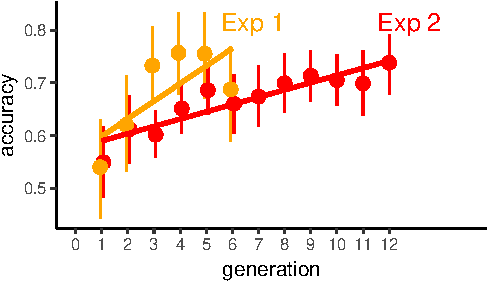
\includegraphics{figs/baseline_bothAccuracy-1} 

}

\caption[Experiments 1 and 2 show increases in accuracy over transmission generations.CHANGE POINT SIZE]{Experiments 1 and 2 show increases in accuracy over transmission generations.CHANGE POINT SIZE}\label{fig:baseline_bothAccuracy}
\end{figure}
\end{CodeChunk}

\begin{CodeChunk}
\begin{figure}[tb]

{\centering 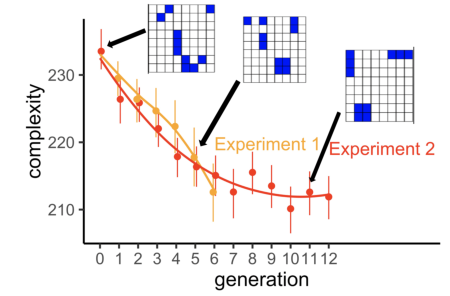
\includegraphics{figs/baseline_bothExp_withplots-1} 

}

\caption[Experiments 1 and 2 show decreases in algorithmic complexity over time]{Experiments 1 and 2 show decreases in algorithmic complexity over time. Grid patterns as produced by participants at generations 0 (initial), 5, and 11 are shown.}\label{fig:baseline_bothExp_withplots}
\end{figure}
\end{CodeChunk}

\section{Experiment 2: Replication and extension of Experiment
1}\label{experiment-2-replication-and-extension-of-experiment-1}

Experiment 2, replicated the task from Experiment 1 with the addition of
twice as many chains and generations. We replicated the task with a
larger sample in order to approximate the shape of the algorithmic
complexity curve. Particularly, we were interested in whether complexity
asymptoted over generations.

\subsection{Method}\label{method-1}

\subsection{Participants}\label{participants-1}

Participants in Experiment 2 were 519 adults recruited on Amazon
Mechanical Turk. These participants were dived into forty diffusion
chains, each of which had twelve generations. Each participant gave
informed consent, and was compensated with \$0.50 for their
participation.

\subsection{Design and Procedure}\label{design-and-procedure-1}

The task in Experiment 2 was identical to Experiment 1. Participants
were told to reproduce patterns on a grid, and their responses were
passed to the next subject in the transmission chain.

Approximately 8\% (n=39) of participants in Experiment 2 were excluded
from analysis due to failure to meet accuracy requirements on the
practice trials or failure to select the complete number of targets on
one or more experimental trials. This resulted in a total of 480
participants included in the analysis.

\subsection{Results}\label{results-1}

The results of this experiment replicated those found in Experiment 1.
Reproduction accuracy increased significantly over generations
(\(\beta =\) 0.051, \(t =\) 4.378, \(p =\) \textless{} .001). Figure
\ref{fig:baseline_bothAccuracy} shows the results for accuracy.

Figure \ref{fig:baseline_bothExp_withplots} shows the results for
algorithmic complexity. Algorithmic complexity appeared to follow
(W.C.??) an exponential function of the form \(y = e^{-x} + b\). We
therefore fit an exponential mixed-effects regression model predicting
complexity from fixed effects of generation and trial number, and random
intercepts for participant, chain, and initial grid (e.g.
\texttt{log(complexity) $\sim$ generation + trial + (1|subject) + (1|initial) + (1|chain)}).
Algorithmic complexity decreased and asymptoted over generations
(\(\beta_{BDM} =\) -0.039, \(t =\) -5.202, \(p =\) \textless{} .001).
Similar trends were also found with chunking and edge length, the
alternate measures of complexity (CHECK THESE MODELS B/C THE LOG
EXPONENTIAL DOESN'T WORK \(\beta_{chunking} =\) -0.834, \(t =\) -14.47,
\(p =\) \textless{} .001; \(\beta_{edge} =\) -1.601, \(t =\) -10.872,
\(p =\) \textless{} .001).

\section{Experiment 3: Introducing an
interlocutor}\label{experiment-3-introducing-an-interlocutor}

In order to add an element of feedback from a more experienced
interlocutor to the iterated-learning process, we adapted the task from
Experiments 1 and 2 to include a secondary, ``editing'' participant.
This participant was analogus to a caregiver who protects their child
from learning incorrect forms of language.

\subsection{Method}\label{method-2}

\subsection{Participants}\label{participants-2}

Participants in Experiment 3 were 1031 adults recruited on Amazon
Mechanical Turk. These participants were dived into forty diffusion
chains, each of which had twelve generations. Each participant gave
informed consent, and was compensated with \$0.50 for their
participation.

\subsection{Design and Procedure}\label{design-and-procedure-2}

In the third, dyad experiment, a primary participant was designated to
be a ``learner'', and completed the same task as in Experiment 1 and
Experiment 2. They were told to re-produce patterns on a grid. A
secondary participant -- the ``fixer'' -- was given an adapted task.
Throughout the study, fixers were not told to re-create patterns, but to
fix patterns to resemble a target grid exactly. Fixers in this
experiment viewed the same target grid as learners, but instead of
seeing an empty input grid, they saw a grid with 10 elements filled in
-- the elements that the previous learner had submitted. The participant
could then edit the 10 items' positions. There was no ``reset'' button
during this task, so produced patterns reflect participants' initial
instincts.

In Experiment 3, a generation consisted of a learner, who re-created the
target grid, and a fixer, who then received the same target grid as well
as the learner's input grid to edit. The fixer's edited pattern was used
as the target grid for the subsequent generation.

Approximately 8\% (n=71 of participants in Experiment 3 were excluded
from analysis due to failure to meet accuracy requirements on the
practice trials or failure to select the necessary number of targets on
one or more experimental trials. This resulted in a total of 960
participants included in the analysis.

\subsection{Analysis and Results}\label{analysis-and-results}

As in Experiments 1 and 2, our primary measures of analysis were
accuracy and complexity. These measures were computed using the same
methods as in the previous experiments.

Fixers and learners had significantly different pattern reproduction
accuracies \ref{fig:dyad_accuracy}. According to a linear mixed-effects
model (need to put in formula? Did an lmer with gen and condition
(learner/fixer) as fixed effects, with all the same random effects), the
accuracies between groups were sigificantly different
(\(\beta_{condition-child} =\) -0.076, \(t =\) -8.956, \(p =\)
\textless{} .001). The fixers' transmission accuracies did not increase
significantly over generations (\(\beta_{fixers} =\) -0.011, \(t =\)
-1.075, \(p =\) .283), while the accuracy of the learners showed a
marginally significant increase (\(\beta_{learners} =\) 0.019, \(t =\)
1.855, \(p =\) .064).

\ref{fig:dyad_complexity} shows the relationship between the complexity
of fixers' and learners' patterns. In each generation, the learner
decreases the complexity of the pattern, and the fixer is able to
compensate for some of this loss. AS in Experiment 2, we fit an
exponential model to the data. Both conditions show decreases in pattern
complexity over generations (\(\beta_{learners} =\) -0.032, \(t =\)
-4.739, \(p =\) \textless{} .001; \(\beta_{fixers} =\) -0.021, \(t =\)
-4.12, \(p =\) \textless{} .001), although the effect of generation is
stronger for learners compared to fixers (\(\beta_{generation} =\)
-5.236, \(t =\) -9.363, \(p =\) \textless{} .001). These results hold
true for all three measures of complexity (Do i need to report all of
these stats??).

\ref{fig:both_complexity} shows that the presence of an editor does help
retain complexity in the grid patterns. The addition of a fixer into the
task allowed a higher degree of complexity to be retained in the
language over time (\(\beta_{condition-child} =\) -3.574, \(t =\)
-5.357, \(p =\) \textless{} .001). Additionally, it appeared that the
patterns in the dyad condition asymptoted sooner than in the baseline
condition (Stats for this?).

\begin{CodeChunk}
\begin{figure}[tb]

{\centering 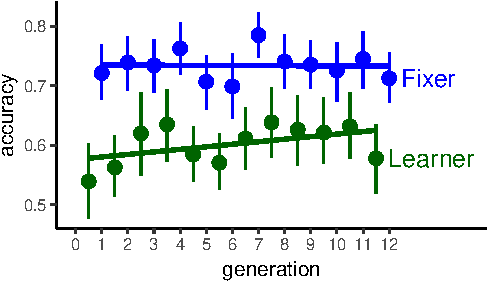
\includegraphics{figs/dyad_accuracy-1} 

}

\caption[In the dyad task, reproduction accuracy stays relatively constant across generations]{In the dyad task, reproduction accuracy stays relatively constant across generations. Fixers have significantly higher accuracies than learners. CHANGE POINT SIZE}\label{fig:dyad_accuracy}
\end{figure}
\end{CodeChunk}

\begin{CodeChunk}
\begin{figure}[tb]

{\centering 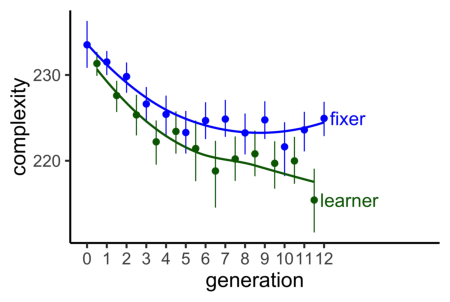
\includegraphics{figs/dyad_complexity-1} 

}

\caption[Fixers reintroudce algorithmic complexity which is lost by learners in the dyad condition]{Fixers reintroudce algorithmic complexity which is lost by learners in the dyad condition.}\label{fig:dyad_complexity}
\end{figure}
\end{CodeChunk}

\begin{CodeChunk}
\begin{figure}[tb]

{\centering 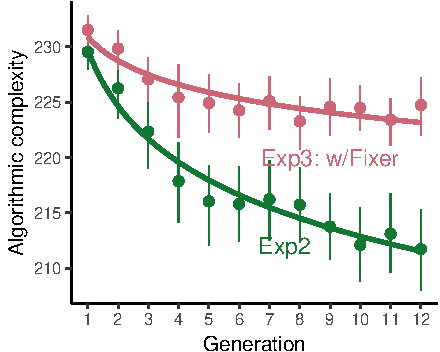
\includegraphics{figs/both_complexity-1} 

}

\caption[The presence of a fixer in the dyad condition causes a much greater level of algorithmic complexity to be retained across the evolution of a novel language]{The presence of a fixer in the dyad condition causes a much greater level of algorithmic complexity to be retained across the evolution of a novel language. CHANGE POSITION IN PAPER}\label{fig:both_complexity}
\end{figure}
\end{CodeChunk}

\section{General Discussion}\label{general-discussion}

Although Experiments 1-3 used a non-linguistic task, we were able to
measure change in a culturally-transmitted, learned symbol system. In
Experiments 1 and 2, language simplified rapidly and dramatically,
reflecting the strong pressure towards simplification in language
learning. These findings replicated those of Kempe et al. (2015): when
transmitting an artifical language of grid patterns, complexity in the
language was lost.

However, the results of Experiment 3 show that this loss is not
permanent, but can be reintroduced in the language by way of a secondary
participant who helps bring the language towards a stable level of
complexity. When the iterated-learning process begins to resemble the
true process of language-learning, where children speak with and are
subject to correction by those more competent in the language, a lesser
amount of complexity was lost during transmission. Additionally, this
stable level of complexity is much higher, and is reached earlier in the
transmission chain with the help of a fixing participant. This stability
in complexity did not mean that the language stopped changing, but that
the descriptiveness and transmissibility pressures were in balance.
Fixers in Experiment 3 represented caregivers -- they were more accurate
at reproducing the language, and could therefore be seen as more fluent
speakers of the language, just as adults are of their native languages.
The learners, on the other hand, had a more difficult task, which
greater strained their working memories, similar to the strain on a
child language learner who is inundated with new words each day. The
fixer's corrected language was passed to the next learner in the chain,
representing a child who, after many years of being corrected by their
own parent, becomes a parent, and, in turn, passes their optimal
language to the next generation. Due to the higher accuracy by fixers,
and therefore greater knowledge of the language, the fixers were were
able to compensate for some (not all) of the loss in complexity seen by
the learners by editing their patterns.

In Experiment 3, the learner's reproduction accuracies were actually
increasing over generations. Despite the stable level of complexity,
learners found the language easier to reproduce over evolution. Although
a high level of descriptiveness was retained in the language,
transmissibility was increasing, without the simplicity pressure
weighing in. Perhaps the language was becoming stable and complex, with
the symbol-patterns changing to be both descriptive and useful, while
being easily transmissible. This reflects the optimal evolutionary
response to these two competing pressures.

When a caregiver or teacher prevents their child from growing up to
believe that ``baba'' is the word for both ``bottle'' and ``sheep'',
they are not only helping their individual child become a competent
speaker of the language, but they are also re-introducing complexity,
and helping the language system as a whole from simplifying to disuse.
Data collection is ongoing with children ages 6-8 at a local science
museum in both the Experiment 2 and Experiment 3 tasks, in order to
investigate whether the pressures of similarity and complexity affect
children similarly to how they affect adults in early language-learning
conditions.

We do not learn language as passive listeners, who absorb a proportion
of the the linguistic input they hear. Therefore, we cannot measure
language learning only through measuring input, nor through measuring
only linguistic output. Languages are both learned and changed through
conversations, with feedback and error correction, to evolve to the
needs of the language's users. Therefore, we must study language
learning in process, to see how it adapts and evolves with communicative
interactions.

\vspace{1em}
\fbox{\parbox[b][][c]{7.3cm}{\centering All code for these analyses are available at\ \url{https://github.com/mcmeyers/iteratedlearning}}}

\section{Acknowledgements}\label{acknowledgements}

This research was funded by a James S. McDonnell Foundation Scholar
Award to DY.

\section{References}\label{references}

\setlength{\parindent}{-0.1in} \setlength{\leftskip}{0.125in}

\noindent

\hypertarget{refs}{}
\hypertarget{ref-bowerman-1982}{}
Bowerman, M. (1982). U shaped behavioral growth. In (pp. 101--145).
Academic Press.

\hypertarget{ref-brentari-2013}{}
Brentari, D., \& Coppola, M. (2013). What sign language creation teaches
us about language. \emph{WIREs Cognitive Science}, \emph{4}(201-211).

\hypertarget{ref-chouinard-2003}{}
Chouinard, M. M., \& Clark, E. V. (2003). Adult reformulations of child
errors as negative evidence. \emph{Journal of Child Language},
\emph{30}(3), 637--669.

\hypertarget{ref-christiansen-2003}{}
Christiansen, M. H., \& Kirby, S. (2003). Language evolution. In M. H.
Christiansen \& S. Kirby (Eds.), (pp. 1--15). Oxford University Press.

\hypertarget{ref-ellis-2008}{}
Ellis, N. C. (2008). The dynamics of second language emergence: Cycles
of language use, language change, and language acquisition. \emph{The
Modern Language Journal}, \emph{92}(ii), 232--249.

\hypertarget{ref-gauvrit-2017}{}
Gauvrit, N., Soler-Toscano, F., \& Guida, A. (2017). A preference for
some types of complexity comment on ``perceived beauty of random texture
patterns: A preference for complexity''. \emph{Acta Psychologica},
\emph{174}, 48--53.

\hypertarget{ref-hudsonkam-2005}{}
Hudson Kam, C. L., \& Newport, E. L. (2005). Regularizing unpredictable
variation: The roles of adult and child learners in languagae formation
and change. \emph{Language Learning and Development}, \emph{1}(2),
151--195.

\hypertarget{ref-kempe-2015}{}
Kempe, V., Gauvrit, N., \& Forsyth, D. (2015). Structure emerges faster
during cultural transmission in children than in adults.
\emph{Cognition}, \emph{136}, 247--254.

\hypertarget{ref-kirby-2007}{}
Kirby, S., Dowman, M., \& Griffiths, T. L. (2007). Innateness and
culture in the evolution of language. \emph{Proceedings of the National
Academy of Sciences}, \emph{104}(12), 5241--5245.

\hypertarget{ref-kirby-2014}{}
Kirby, S., Griffiths, T., \& Smith, K. (2014). Iterated learning and the
evolution of language. \emph{Current Opinion in Neurobiology},
\emph{28}, 108--114.

\hypertarget{ref-lupyan-2010}{}
Lupyan, G., \& Dale, R. (2010). Language structure is partly determined
by social structure. \emph{PLoS ONE}, \emph{5}(1), 1--10.

\hypertarget{ref-penner-1987}{}
Penner, S. G. (1987). Parental responses to grammatical and
ungrammatical child utterances. \emph{Child Development}, \emph{58}(2),
376--384.

\hypertarget{ref-raviv-2018}{}
Raviv, L., \& Arnon, I. (2018). Systematicity, but not compositionality:
Examining the emergence of linguistic structure in children and adults
using iterated learning. \emph{Cognition}, \emph{181}, 160--173.

\hypertarget{ref-romberg-2010}{}
Romberg, A. R., \& Saffran, J. (2010). Statistical learning and language
acquisition. \emph{WIREs Cognitive Science}, \emph{1}, 906--914.

\hypertarget{ref-sandler-2005}{}
Sandler, W., Meir, I., Padden, C., \& Aronoff, M. (2005). The emergence
of grammar: Systematic structure in a new language. \emph{Proceedings of
the National Academy of Sciences}, \emph{102}(7), 2661--2665.

\hypertarget{ref-senghas-2003}{}
Senghas, A. (2003). Intergenerational influence and ontogenetic
development in the emergence of spatial grammar in nicaraguan sign
language. \emph{Cognitive Development}, \emph{18}, 511--531.

\hypertarget{ref-smith-2010}{}
Smith, K., \& Wonnacott, E. (2010). Eliminating unpredictable variation
through iterated learning. \emph{Cognition}, \emph{116}, 444--449.

\hypertarget{ref-verhoef-2014}{}
structure, E. of combinatorial, \& signals. (2014). Verhoef, tessa and
kirby, simon and de boer, bart. \emph{Journal of Phonetics}, \emph{43},
57--68.

\hypertarget{ref-zenil-2014}{}
Zenil, H., Soler-Toscano, F., Dingle, K., \& Louis, A. A. (2014).
Correlation of automorphism group size and topolical properties with
program-size complexity evaluations of graphs and complex networks.
\emph{Physica A}, \emph{404}, 341--358.

\bibliographystyle{apacite}


\end{document}
